\documentclass[12pt]{report}
\usepackage[utf8]{inputenc}
\usepackage[russian]{babel}
\usepackage{float}
%\usepackage[14pt]{extsizes}
\usepackage{listings}
\usepackage{comment}
% Для листинга кода:
\usepackage{lipsum}
\usepackage{indentfirst}
\setlength{\parindent}{5ex}
\setlength{\parskip}{1em}
% Для измененных титулов глав:
\usepackage{titlesec, blindtext, color} % подключаем нужные пакеты
\definecolor{gray75}{gray}{0.75} % определяем цвет
\newcommand{\hsp}{\hspace{20pt}} % длина линии в 20pt
% titleformat определяет стиль
\titleformat{\chapter}[hang]{\Huge\bfseries}{\thechapter\hsp\textcolor{gray75}{|}\hsp}{0pt}{\Huge\bfseries}


% plot
\usepackage{pgfplots}
\usepackage{filecontents}
\usetikzlibrary{datavisualization}
\usetikzlibrary{datavisualization.formats.functions}
\begin{filecontents}{bubble_straight.dat}
0 0
200  0.0 
400 0.00001
600 0.0002
800 0.0003
1000 0.0004
\end{filecontents}
\begin{filecontents}{insert_straight.dat}
0 0
200  0.0001 
400 0.003
600 0.01099
800 0.01099
1000 0.01099
\end{filecontents}
\begin{filecontents}{quick_straight.dat}
0  0.0 
200  0.0002
400 0.0003
600 0.003
800 0.01099
1000 0.01099
\end{filecontents}

\begin{filecontents}{bubble_rev.dat}
0 0
200  0.0009697
400 0.00101
600 0.002792
800 0.007021
1000 0.010028
\end{filecontents}
\begin{filecontents}{insert_rev.dat}
0 0
200  0.000605
400 0.00500
600 0.007987
800 0.011032
1000 0.019666
\end{filecontents}
\begin{filecontents}{quick_rev.dat}
0 0
200  0.000605
400 0.007000
600 0.010987
800 0.015032
1000 0.026696
\end{filecontents}

\begin{filecontents}{bubble_rand.dat}
0 0
200  0.000505
400 0.00300
600 0.004987
800 0.009032
1000 0.01666
\end{filecontents}
\begin{filecontents}{insert_rand.dat}
0 0
200  0.0 
400 0.000504
600 0.001192
800 0.0029708
1000 0.0044880
\end{filecontents}
\begin{filecontents}{quick_rand.dat}
0 0
200  0.0 
400 0.000997
600 0.003843
800 0.005000
1000 0.00845
\end{filecontents}
\usepackage{pdfpages}
\usepackage{graphicx}
\graphicspath{{src/}}
\DeclareGraphicsExtensions{.pdf,.png,.jpg}

\begin{document}
\lstset{ %
language=Python,                 % выбор языка для подсветки (здесь это С)
basicstyle=\small\sffamily, % размер и начертание шрифта для подсветки кода
numberstyle=\tiny,           % размер шрифта для номеров строк
stepnumber=1,                   % размер шага между двумя номерами строк
numbersep=3pt,                % как далеко отстоят номера строк от подсвечиваемого кода
backgroundcolor=\color{white}, % цвет фона подсветки - используем \usepackage{color}
showspaces=false,            % показывать или нет пробелы специальными отступами
showstringspaces=false,      % показывать или нет пробелы в строках
showtabs=false,             % показывать или нет табуляцию в строках
frame=single,              % рисовать рамку вокруг кода
tabsize=2,                 % размер табуляции по умолчанию равен 2 пробелам
captionpos=t,              % позиция заголовка вверху [t] или внизу [b] 
breaklines=true,           % автоматически переносить строки (да\нет)
breakatwhitespace=false, % переносить строки только если есть пробел
escapeinside={\%*}{*)},   % если нужно добавить комментарии в коде
}
%\def\chaptername{} % убирает "Глава"
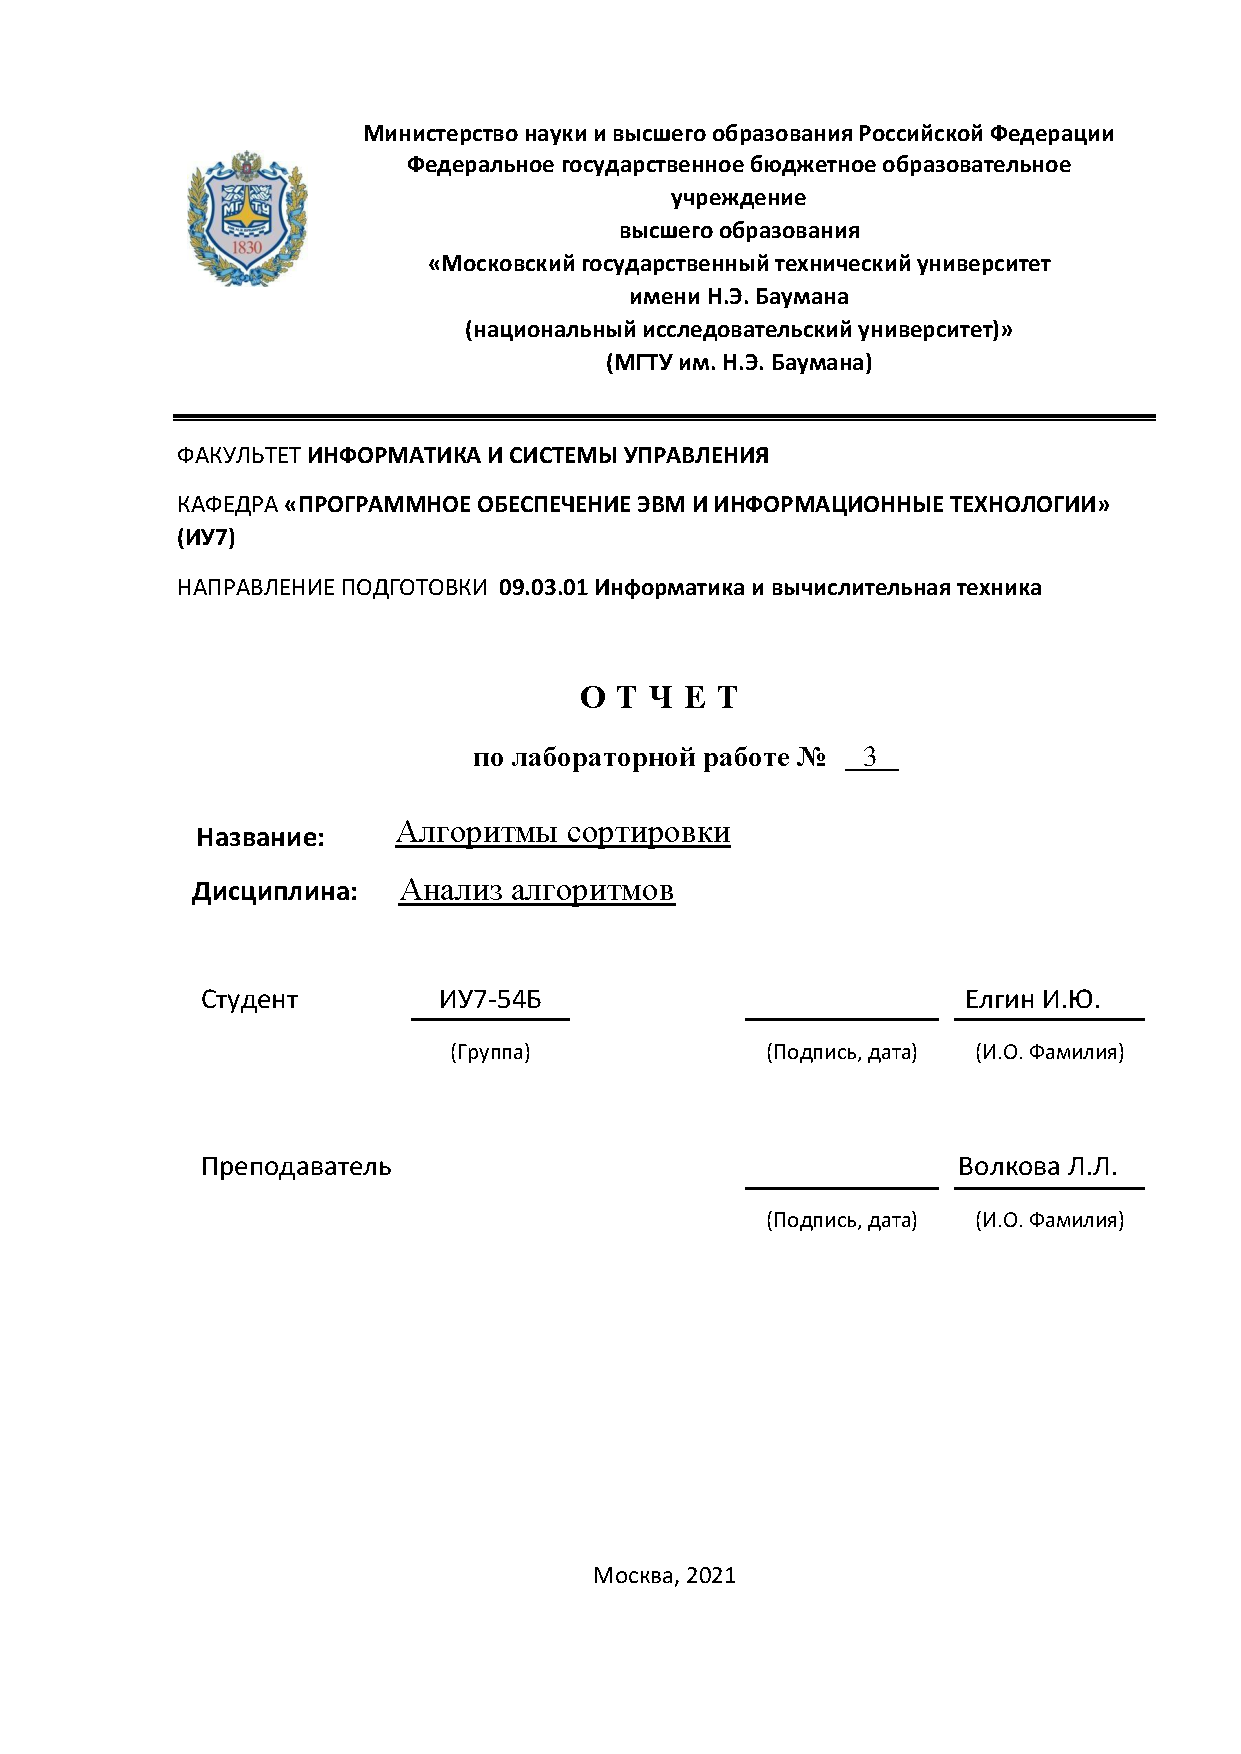
\includepdf[pages=1]{titul.pdf}
\bibliographystyle{9}
\renewcommand{\contentsname}{Содержание}
\tableofcontents

\newpage
\chapter*{Введение}
\addcontentsline{toc}{chapter}{Введение}
Алгоритмы сортировки часто применяются в практике программирования. В том числе в областях связанных с математикой, физикой, компьютерной графикой и т.д.

На сегодняшний день существует не одна вариация алгоритмов сортировки. Все они различаются по скорости сортировки и по объему необходимой памяти. 
Цель данной лабораторной работы - обучение расчету трудоемкости алгоритмов
Для достижения поставленой цели необходимо осуществить следующие задачи:
\begin{enumerate}
\item Разработать и реализовать алгоритмы трёх различных сортировок;
\item Провести тестирование алгоритмов по времени на данных являющихся худшим, лучшим и обычным случаем для данного алгоритма;
\item По результатам проделанной работы сделать выводы и написать отчёт.
\end{enumerate}
\chapter{Аналитическая часть}
Выберем три алгоритма сортировок для реализации.
\section{Сортировка пузырьком}
Алгоритм состоит из повторяющихся проходов по сортируемому массиву. За каждый проход элементы последовательно сравниваются попарно и, если порядок в паре неверный, выполняется обмен элементов.

В данную сортировку может быть добавлен флаг показывающий происходила ли перестановка при очередном проходе. Если перестановки не происходило то массив отсортирован и мы можем завершить алгоритм.

\section{Сортировка вставками}
На каждом шаге выбирается один из элементов неотсортированной части массива (максимальный/минимальный) 
и помещается на нужную позицию в отсортированную часть массива. 

При этом часть массива от позичии вставки до позиции взятия элемента сдвикается на 1 .

\section{Сортировка шейкером}
Алгоритм данной сортировки схож с алгоритмом сортировки пузырьком. Мы проходимся по масиву сравниваем два соседних элемента, если порядок в паре неверный, выполняется обмен элементов. Однако в данном алгоритме мы чередуеми проходы по масиву в одну и в другую сторону.

\section{Вывод}
В качестве алгоритмов сортировок для реализации были выбраны сортировка пузырьком, сортировка вставками и сортировка шейкером.

\chapter{Конструкторская часть}
\section{Схемы алгоритмов}
В данном разделе будут рассмотрены схемы алгоритмов пузырьком с флагом (\ref{ris:imageSB}), сортировки вставками (\ref{ris:imageIS}), сортировки шейкером (\ref{ris:imageQS}).

\begin{figure}[H]
\center{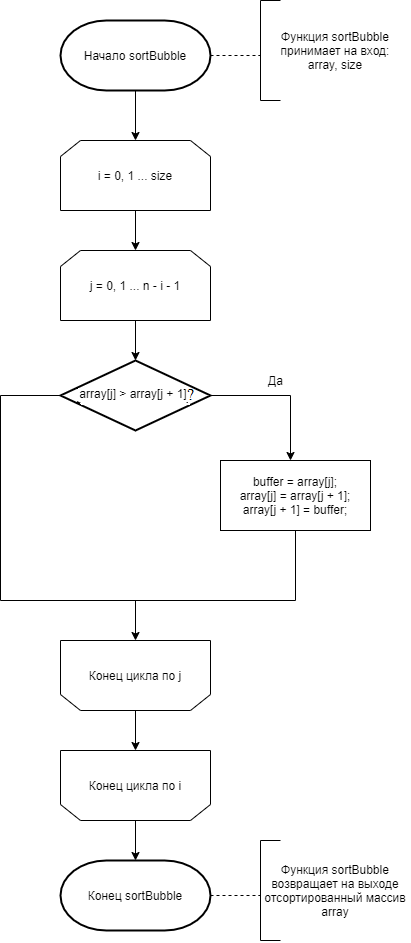
\includegraphics[height = 18cm]{schem/scheme_bubble.png}}
\caption{Схема алгоритма сортировки пузырьком}
\label{ris:imageSB}
\end{figure}

\newpage
\begin{figure}[H]
\center{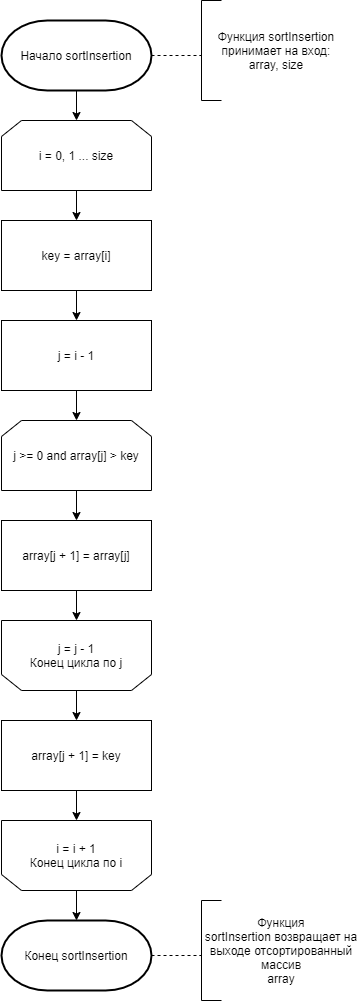
\includegraphics[height = 18cm]{schem/scheme_insert.png}}
\caption{Схема алгоритма сортировки вставками}
\label{ris:imageIS}
\end{figure}

\newpage
\begin{figure}[H]
\center{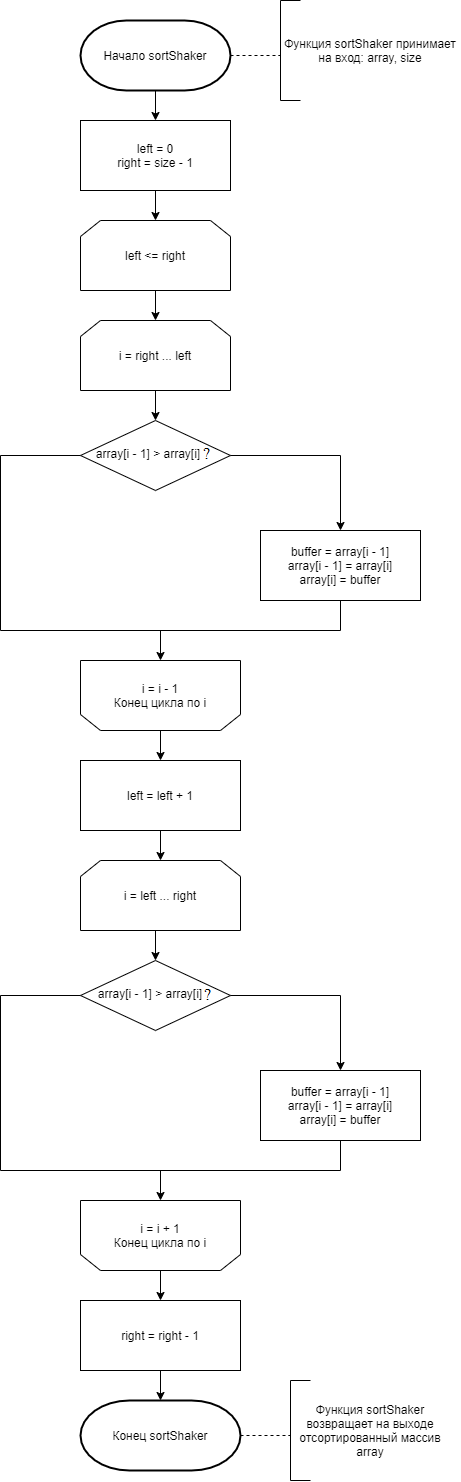
\includegraphics[height = 18cm]{schem/scheme_shaker.png}}
\caption{Схема алгоритма сортировки шейкером}
\label{ris:imageQS}
\end{figure}

\section{Трудоемкость алгоритмов}
Введем модель трудоемкости для оценки алгоритмов:
\begin{enumerate}
  	\item  базовые операции стоимостью 1: $ +, -, =, ==, <=, >=, !=, +=, -=, [], ++, --, and, !, or$ получение полей класса
  	\item  базовые операции стоимостью 2: $ *, /, /=, *=$
	\item оценка трудоемкости цикла: $$Fц = a + N*(a + Fтела)$$, где $a$ - условие цикла
	\item стоимость условного перехода возьмем за 0, стоимость вычисления условия остаётся.
\end{enumerate}

Далее будет приведены оценки трудоемкости алгоритмов.

\subsection{Сортировка вставками}

\textbf{Лучший случай:} отсортированный массив. При этом все внутренние циклы состоят всего из одной итерации.\newline
Трудоемкость: \begin{equation}T(n) = 4 + 1 + 2n * (2+2+3)  =  2n * 7 = 14n + 1 = O(n)\end{equation}

\textbf{Худший случай:} массив отсортирован в обратном нужному порядке. Каждый новый элемент сравнивается со всеми в отсортированной последовательности.
Все внутренние циклы будут состоять из j итераций. \newline
Трудоемкость: \begin{equation}T(n) = 1+n*(2+2+4n*(4+1)+3) = 2n*n+7n+1 =  O(n^2)\end{equation}

 \subsection{Сортировка пузырьком}
\textbf{Лучший случай:} Массив отсортирован; не произошло ни одного обмена за 1 проход -> выходим из цикла \newline
Трудоемкость:  \begin{equation}1+1+1+1+2n*5+2+1 = 10n + 7=  O(n)\end{equation}

\textbf{Худший случай:}  Массив отсортирован в обратном порядке; в каждом случае происходил обмен\newline
Трудоемкость: \begin{equation}1+1+2n*(1 + 1 + (n-1)/2*(5+1+8 ) ) = 2 + 14n^2 - 10n = O(n^2)\end{equation}

\subsection{Сортировка шейкером}
\textbf{Лучший случай:} Массив отсортирован; не произошло ни одного обмена за 1 проход -> выходим из цикла \newline
Трудоемкость:  \begin{equation}1+2n*(1 + 8 + 5) = 1+28n=  O(n)\end{equation}

\textbf{Худший случай:}  Массив отсортирован в обратном порядке; в каждом случае происходил обмен\newline
Трудоемкость: \begin{equation}1+1+2n * (1 + 1 + 2n*(4+5)) = 2 + 4n + 36 n*n = O(n^2)\end{equation}


\section{Вывод}
Сортировка пузырьком: лучший - $O(n)$, худший - $O(n^2)$ \newline
Сортировка вставками: лучший - $O(n)$, худший - $O(n^2)$ \newline
Cортировка шейкером: лучший - $O(n)$, худший - $O(n^2)$ \newline

\chapter{Технологическая часть}
\section{Выбор ЯП}
В качестве языком программирования мною выбран язык Python, так как я имею опыт работы с данным языком программирования, Pyton позволяет удобно работать с масивами.

Время работы алгоритмов было замерено с помощью функции process\_time() из библиотеки time \cite{lit2}.


\section{Описание структуры ПО}
Программа состоит из одного файла main.py в котором находятся функции алгоритмов сортировок.

\section{Сведения о модулях программы}
\newpage
\begin{lstlisting}[label=some-code,caption=Сортировка пузырьком]
def BubbleSort(array, n):
    fl = 1
    for i in range(0, n - 1):
        if fl :
            fl = 0
            for j in range(1, n - i):
                if (array[j-1] > array[j]):
                    fl = 1
                    array[j], array[j - 1] = array[j - 1], array[j] 
        else:
            break;
\end{lstlisting}

\begin{lstlisting}[label=some-code,caption=Сортировка вставками]
def InsertionSort(array, n):
    for i in range(0, n - 1):
        b = array[i]
        j = i - 1
        while j >=0 and b < array[j] :
            array[j+1] = array[j]
            j -= 1
        array[j+1] = b
\end{lstlisting}
\newpage
\begin{lstlisting}[label=some-code,caption=Сортировка шейкером]
def ShakerSort(array, n): 
    f = 1
    s = 0
    e = n - 1
    while f: 
        swapped = False 
        for i in range(s, e): 
            if (array[i] > array[i + 1]) : 
                array[i], array[i + 1] = array[i + 1], array[i] 
                f = 1
        if not(f): 
            break
        f = 0
        e -= 1
        for i in range(e, s, -1): 
            if (array[i] > array[i + 1]):
                array[i], array[i + 1] = array[i + 1], array[i] 
                f = 1
        s = s + 1
\end{lstlisting}
\section{Вывод}
В качестве языка программирования для реализации алгоритмов сортировки был выбран Python. На данном языке програмирования были написаны функции сортировок и функция тестирования сортировок по времени.

\chapter{Исследовательская часть}

Был проведен замер времени работы каждой из сортировок на худших лучших и случайных данных.
\section{Постановка эксперемента}
Лучшим случаем для всех трёх сортировок будет массив отсортированный в нужном порядке, так как он совпадает с результатом и никаких действий над ним производить не нужно.

Худшим случаем для сортировки пузырьком является обратно отсортированный масив так как для полной отсортировки каждый эллемент должен проделать путь от в i элементов где i позиция элементов. А за один проход на место будет перемещатся только один элемент.

Худшим случаем для сортировки вставками является обратно отсортированный масив \cite{lit1}.

Худшим случаем для сортировки шейкером является обратно отсортированный масив. По анологии с сортировкой пузырьком, только здесь будут чередоваться перемещения наибольшего и наименьшего элемента.
\subsection{Сортировка пузырьком}
В таблице 4.1 представлен результат работы сортировки на массивох разных длин, для худщих лучших и случайных данных.
\begin{table}[h!]
	\begin{tabular}{|c|c|c|c|}
	len & Отсортированный, сек. & Обратный порядок, сек. & Случайный,сек \\ [0.5ex] 
 	\hline\hline
 	200 & 0.0 & 0.0015225 & 0.0 \\
 	\hline
 	400 & 0.0 & 0.003125 & 0.0015625\\
 	\hline
	600 & 0.0 & 0.0046875 & 0.003125 \\
	\hline
	800 & 0.0 & 0.0078125 & 0.0046875 \\
	\hline
	1000 & 0.0015625 & 0.0125 & 0.0109375\\
	\hline
	\end{tabular}
	\caption{Время работы сортировки пузырьком}
\end{table}


\subsection{Сортировка вставками}
В таблице 4.2 представлен результат работы сортировки на массивох разных длин, для худщих лучших и случайных данных.
\begin{table}[h!]
	\begin{tabular}{|c|c|c|c|}
	len & Отсортированный, сек. & Обратный порядок, сек. & Случайный,сек \\ [0.5ex] 
 	\hline\hline
 	200 & 0.0 & 0.0015625 & 0.0 \\
 	\hline
 	400 & 0.0 & 0.0015625 & 0.0015625\\
 	\hline
	600 & 0.0 & 0.00625 & 0.0031250 \\
	\hline
	800 & 0.0 & 0.0140625 & 0.0046750\\
	\hline
	1000 & 0.0 & 0.0352521 & 0.0.0076875\\
	\hline
	\end{tabular}
	\caption{Время работы сортировки вставками}
\end{table}

\subsection{Сортировка шейкером}
В таблице 4.3 представлен результат работы сортировки на массивох разных длин, для худщих лучших и случайных данных.
\begin{table}[h!]
	\begin{tabular}{|c|c|c|c|}
	len & Отсортированный, сек. & Обратный порядок, сек. & Случайный,сек \\ [0.5ex] 
 	\hline\hline
 	200 & 0.0 & 0.0015625 & 0.0015625 \\
 	\hline
 	400 & 0.0 & 0.0046875 & 0.0015625\\
 	\hline
	600 & 0.0 & 0.0125000 &  0.009375\\
	\hline
	800 & 0.0015625 & 0.0.0203125 & 0.0140625\\
	\hline
	1000 & 0.0015625 & 0.034375 & 0.0203225\\
	\hline
	\end{tabular}
	\caption{Время работы сортировки шейкером}
\end{table}

\subsection{Графики времени сортировок}
На данных графиках представлены зависимости времени работы от размера массива для сортировок при лучших, хучших и случайных данных. 
\begin{figure}
\begin{tikzpicture}
\begin{axis}[
    	axis lines = left,
    	xlabel = $len$ эл.,
    	ylabel = {$time$} сек.,
	legend pos=north west,
	ymajorgrids=true
]
\addplot[color=red] table[x index=0, y index=1] {bubble_straight.dat}; 
\addplot[color=green] table[x index=0, y index=1] {insert_straight.dat};
\addplot[color=blue, mark=square] table[x index=0, y index=1] {quick_straight.dat};

\addlegendentry{bubble}
\addlegendentry{insert}
\addlegendentry{shaker}
\end{axis}
\end{tikzpicture}
\caption{Сравнение сортировки уже отсортированных массивов} \label{plot:straight}
\end{figure}
\par
\begin{figure}
    \centering
\begin{tikzpicture}
\begin{axis}[
    	axis lines = left,
    	xlabel = $len$ эл.,
    	ylabel = {$time$} сек.,
	legend pos=north west,
	ymajorgrids=true
]
\addplot[color=red] table[x index=0, y index=1] {bubble_rev.dat}; 
\addplot[color=green] table[x index=0, y index=1] {insert_rev.dat};
\addplot[color=blue, mark=square] table[x index=0, y index=1] {quick_rev.dat};

\addlegendentry{bubble}
\addlegendentry{insert}
\addlegendentry{shaker}
\end{axis}
\end{tikzpicture}
\caption{Сравнение сортировки массивов, отсортированных в обратном порядке} \label{plot:rev}
\end{figure}
\par
\begin{figure}
\begin{tikzpicture}
\begin{axis}[
    	axis lines = left,
    	xlabel = $len$ эл.,
    	ylabel = {$time$} сек.,
	legend pos=north west,
	ymajorgrids=true
]
\addplot[color=red] table[x index=0, y index=1] {bubble_rand.dat}; 
\addplot[color=green] table[x index=0, y index=1] {insert_rand.dat};
\addplot[color=blue, mark=square] table[x index=0, y index=1] {quick_rand.dat};

\addlegendentry{bubble}
\addlegendentry{insert}
\addlegendentry{shaker}
\end{axis}
\end{tikzpicture}
\caption{Сравнение сортировки случайных массивов} \label{plot:rand}
\end{figure}
\newpage
\subsection{Вывод}
Были протестированы алгоритмы сортировки на массивах размерами 200…1000 с шагом 200. Рассмотрены отсортированные, отсортированные в обратном порядке массивы и массивы со случайными значениями.

В результате тестирования было получено, что лучшее время сортировки показывают на отсортированных массивах. Худшие значения сортировки показывают на обратно отсортированных массивах, причём чем больше размер такого массива, тем медленнее работают сортировки. 

При сравнении времени работы алгоритмов можно сделать вывод, что на размерах массива до 400 элементов время работы алгоритмов приближено к 0 сек. При работе с массивами размерами более 400 элементов сортировка пузырьком показывает наихудший результат. При сортировки случайных массивов лучшее время показывает сортировка вставками.

\chapter*{Заключение}
\addcontentsline{toc}{chapter}{Заключение}
В ходе выполнения данной лабораторной работы были реализованы три алгоритма сортировки: сортировка пузырьком, сортировка вставками и быстрая сортировка. Был проведён анализ каждого алгоритма и измерено время работы алгоритмов для массивов разных размеров. Была оценена трудоёмкость алгоритмов.

Лучшее время работы все сортировки показывают на отсортированных массивах. Худшее время алгоритмы сортировки показали при работе с массивами, отсортированными в обратном порядке. Причём в худшем случае зависимость времени работы от размера массива квадратичная.

Был сделан вывод, что на размерах массива до 400 элементов время работы алгоритмов приближено к 0 сек. При работе с массивами размерами более 400 элементов сортировка пузырьком показывает наихудший результат. При сортировки случайных массивов лучшее время показывает сортировка вставками.


\addcontentsline{toc}{chapter}{Литература}
\begin{thebibliography}{4}
	\bibitem{lit3}  Кормен, Т., Лейзерсон, Ч., Ривест, Р., Штайн, К. Глава 7. Быстрая сортировка // Алгоритмы: построение и анализ = Introduction to Algorithms / Под ред. И. В. Красикова. — 2-е изд. — М.: Вильямс, 2005.
    \bibitem{lit4} Левитин А. В. Глава 4. Метод декомпозиции: Быстрая сортировка // Алгоритмы. Введение в разработку и анализ — М.: Вильямс, 2006.
    
    \bibitem{lit1} Алгоритм сортировки вставками $[$Электронный ресурс$]$. – Режим доступа:$https://www.quora.com/What-is-the-worst-case-example-of-selection-sort-and-insertion-sort$ (дата обращения 10.10.21)
    
    \bibitem{lit2} Сортировка всавками $[$Электронный ресурс$]$. – Режим доступа:$https://studopedia.ru/9_97870_sortirovka-vstavkami.html$ (дата обращения 10.10.21)
    
\end{thebibliography}

\end{document}
